% Generated by pipeline/paper/scripts/make_result_figures.py. Do not edit by hand.
% 1000G chr22 CEU. Recall of the variant key in the new sample. The last bar is the union.
% Shared figure style. Input once; a second input is a no-op.
\ifdefined\actsplotsready
\else
  \def\actsplotsready{1}
  \colorlet{actsteal}{teal!72!black}
  \colorlet{actstealfaint}{teal!16}
  \colorlet{actsorange}{orange!88!black}
  \colorlet{actsink}{black!80}
  \colorlet{actsghost}{black!45}
  \colorlet{actsfail}{red!62!black}
  \colorlet{actsrule}{black!50}
  \usetikzlibrary{intersections}
  \usepgfplotslibrary{fillbetween,groupplots}
  \pgfplotsset{
    acts/.style={
      font=\scriptsize\sffamily,
      tick label style={font=\scriptsize\sffamily},
      label style={font=\scriptsize\sffamily},
      legend style={
        font=\scriptsize\sffamily,
        draw=none,
        fill=none,
        cells={anchor=west},
        inner sep=1pt,
        column sep=6pt
      },
      legend cell align=left,
      scale only axis,
      clip=false,
      axis line style={actsrule},
      tick style={actsrule},
      tick align=outside,
      axis lines=left,
      xmajorgrids=true,
      major grid style={black!7},
      ymajorgrids=false,
      every node/.append style={font=\scriptsize\sffamily, inner sep=1.5pt},
      every axis plot/.append style={line join=round, line cap=round},
    },
  }
  \tikzset{
    actlab/.style={
      font=\scriptsize\sffamily,
      fill=white,
      fill opacity=0.92,
      text opacity=1,
      inner sep=1.35pt,
      outer sep=0.5pt,
    },
  }
\fi

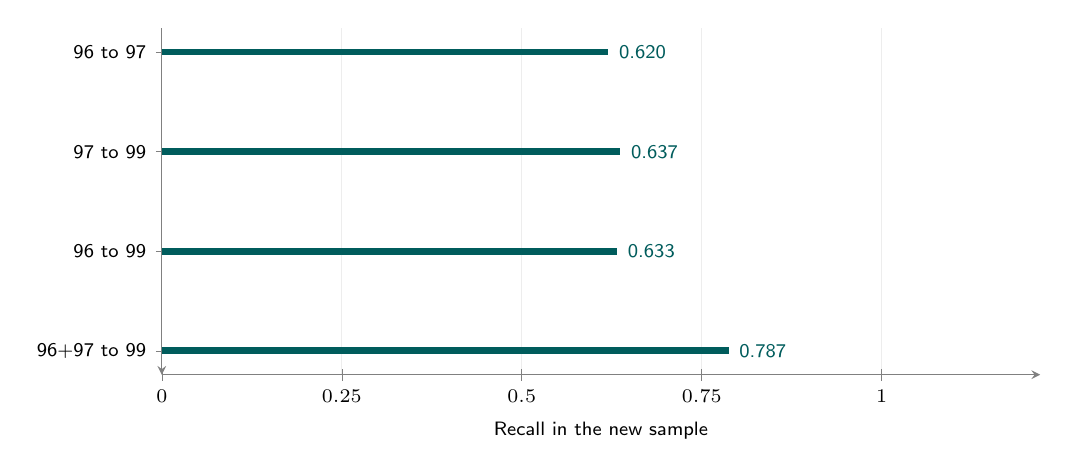
\begin{tikzpicture}
\begin{axis}[
  acts,
  width=0.92\columnwidth,
  height=4.40cm,
  xmin=0, xmax=1.22,
  xtick={0,0.25,0.5,0.75,1},
  xlabel={Recall in the new sample},
  symbolic y coords={r0,r1,r2,r3},
  ytick={r0,r1,r2,r3},
  y dir=reverse,
  yticklabels={{96 to 97},{97 to 99},{96 to 99},{96+97 to 99}},
  enlarge y limits=0.08,
]
\addplot[draw=none, forget plot] coordinates {(0,r0) (0,r1) (0,r2) (0,r3)};
% source: vep_chr22_overlap.json rows.recall_in_new and growing_cohort.recall_in_new
\draw[actsteal, line width=2.4pt, line cap=butt] (axis cs:0,r0) -- (axis cs:0.620406,r0);
\node[actlab, anchor=west, text=actsteal, xshift=2pt] at (axis cs:0.620406,r0) {0.620};
\draw[actsteal, line width=2.4pt, line cap=butt] (axis cs:0,r1) -- (axis cs:0.636935,r1);
\node[actlab, anchor=west, text=actsteal, xshift=2pt] at (axis cs:0.636935,r1) {0.637};
\draw[actsteal, line width=2.4pt, line cap=butt] (axis cs:0,r2) -- (axis cs:0.632661,r2);
\node[actlab, anchor=west, text=actsteal, xshift=2pt] at (axis cs:0.632661,r2) {0.633};
\draw[actsteal, line width=2.4pt, line cap=butt] (axis cs:0,r3) -- (axis cs:0.787397,r3);
\node[actlab, anchor=west, text=actsteal, xshift=2pt] at (axis cs:0.787397,r3) {0.787};
\end{axis}
\end{tikzpicture}
